\documentclass[a4paper, 12pt, twoside, openright]{book}
\addtolength{\oddsidemargin}{+1.3cm}
\addtolength{\evensidemargin}{-1.3cm}
\usepackage[english]{babel}
\usepackage[T1]{fontenc}
\usepackage[utf8]{inputenc}
\usepackage{fancyhdr}
\usepackage{float}
\usepackage{graphicx}
\usepackage{wrapfig}
\usepackage{siunitx} %per scrivere il simbolo °
\usepackage{verbatim} %per i commenti1
\usepackage{subcaption}
\usepackage{amsmath}
\usepackage[linesnumbered, ruled, vlined]{algorithm2e}
\setcounter{secnumdepth}{3}
\setcounter{tocdepth}{6}
\usepackage{multirow}
\usepackage{enumitem}
\usepackage{longtable}
\newcommand{\minitab}[2][l]{\begin{tabular}#1 #2\end{tabular}}
\usepackage{rotating}
\usepackage{url}
\DeclareMathOperator*{\argmax}{arg\,max}
\DeclareMathOperator*{\argmin}{arg\,min}

%\usepackage{booktabs,array}
%\usepackage{tikz}

%\usepackage{tabularx}

%\usepackage{chngcntr}
%\counterwithin{table}{section}

%------------------------------ colors
\usepackage[usenames,dvipsnames,table]{xcolor} % use colors on table and more
\definecolor{333}{RGB}{51, 51, 51} % define custom color
\definecolor{background}{RGB}{255, 254, 213}
\definecolor{comment}{RGB}{17,167,5}
\definecolor{keyword}{RGB}{195,47,8}
\definecolor{string}{RGB}{142,195,0}
\definecolor{number}{RGB}{90,84,84}
\definecolor{identifier}{RGB}{0,90,201}

%------------------------------ source code
\usepackage{listings}

\lstset{
  basicstyle=\footnotesize\sffamily,
  commentstyle=\itshape\color{gray},
  captionpos=b,
  frame=shadowbox,
  language=HTML,
  rulesepcolor=\color{333},
  tabsize=2
}

\lstdefinestyle{code}{
  backgroundcolor=\color{background},
  basicstyle=\footnotesize\sffamily,
  commentstyle=\color{comment},
  frame=L,
  identifierstyle=\color{identifier},
  keywordstyle=\color{keyword},
  numbers=left,
  numbersep=10pt,
  numberstyle=\tiny\color{number},
  stringstyle=\color{string},
  showstringspaces=false,  
  stepnumber=1,
  tabsize=2
}

\usepackage[colorlinks=true, linkcolor=black, citecolor=blue, urlcolor=black]{hyperref}

%------------------------------ define Abstract environment, missing in the 'book' class
\newenvironment{abstract}{\cleardoublepage \null \vfill \begin{center}\bfseries\abstractname \end{center}}{\vfill\null}
\addto\captionsenglish{\renewcommand*\abstractname{Abstract}} % change Abstract title

%------------------------------ active url
\usepackage{url}
\renewcommand{\UrlFont}{\color{black}\small\ttfamily} % active ref
%------------------------------ macros
\newcommand{\sectionname}{Section} % define Section ref
\newcommand{\subsectionname}{Sub-section} % define Sub-section ref
\renewcommand*\arraystretch{1.4} % tables padding

%acronimi
\usepackage[printonlyused]{acronym}

%Rules in tables
\usepackage{booktabs}

%Formatted quote
\newcommand{\myquote}[2]{
\begin{quote}
	\textbf{\Large ``}{\textit{#1}}\textbf{\Large ''}\\
	\textbf{#2}\\\\
\end{quote}
}

%Formatted item with description
\newcommand{\descItem}[2]{
\item{\textbf{#1}\\#2}
}

%Formatted item with description
\newcommand{\myBibItem}[4]{
\bibitem{#1}#2, "#3" in \emph{#4}.
}

\newcommand{\myBibRef}[5]{
\bibitem{#1}#2, \href{#3}{"#4"}, \emph{#5}.
}

%Cell with vertical text
\newcommand{\verticalCell}[2]{
\multirow{#1}{*}{\rotatebox[origin=c]{90}{#2}}
}

%Tab Item Cell
\newcommand{\itemCell}[1]{
\textbullet\ {#1}
}

\begin{document}
\frontmatter
\begin{titlepage} %------------------------------ TITLE PAGE
\begin{center}
\vbox to0pt{\vbox to\textheight{\vfill \includegraphics[width=11.5cm]{./Images/unipd-light} \vfill}\vss}

\begin{minipage}{.20\textwidth}
  \includegraphics[height=2.5cm]{./Images/unipd-bn}
\end{minipage}\begin{minipage}{.90\textwidth}
  \begin{table}[H]
  \begin{tabular}{l}
  \scshape{\Large{\bfseries{University of Padova}}} \\
  \hline
  \scshape{\Large{Engineering~Departement}} \\
  \end{tabular}
  \end{table}
\end{minipage}

\vspace{1cm}
\emph{\Large{Computer~Engineering~Master~Degree}} \\
\vspace{1.5cm}
\scshape{\Large{\bfseries{Invisible CAPPCHA}}} \\
\vspace{0.2cm} \linespread{1} 
\scshape{\large{\bfseries{}}}
\end{center}

\vfill
\begin{normalsize}
\begin{flushleft}
  %\hspace{45pt} \textit{Laureando} \hspace{160pt} \textit{Relatore}\\
  \hspace{65pt} \textit{Candidate} \hspace{130pt} \textit{Supervisor}\\
  \vspace{5pt}
  \hspace{25pt} \large{\textbf{\footnotesize{Di Nardo Di Maio Raffaele}}} \hspace{55pt} \large{\textbf{\footnotesize{Prof. Migliardi Mauro}}}\\
  \vspace{50pt}
  %\hspace{260pt} \normalsize{\textit{Co-relatore}}\\
  \hspace{240pt} \normalsize{\textit{Co-Supervisors}}\\
  \vspace{5pt}
  \hspace{242pt} \large{\textbf{\footnotesize{Guerar Meriem}}}
\end{flushleft}
\end{normalsize}

\vfill
\begin{center}
\textsc{DD-MM-YYYY}
\hspace{-0.2cm}
\line(1, 0){360}

\textsc{Accademic Year 2020-2021}
\end{center}
\end{titlepage}
\cleardoublepage % make left page blank
\thispagestyle{empty}
\null
\vspace{2cm}
\begin{flushright}
 To my parents, that always help\\
me to be happy doing what I love\\
and support me reaching my goals.
\end{flushright}
\vfill
\cleardoublepage % make left page blank
\null
\vspace{2cm}
\thispagestyle{empty}
\myquote{Most people assume that once security software is installed, they're protected. This isn't the case. It's critical that companies be proactive in thinking about security on a long-term basis.}{Kevin Mitnick}
\myquote{You have to learn the rules of the game. And then you have to play better than anyone else.}{Albert Einstein}
\myquote{Si come il ferro s'arrugginisce sanza esercizio, e l'acqua si putrefà o nel freddo s'addiaccia, così lo 'ngegno sanza esercizio si guasta.}{Leonardo da Vinci}
\vfill
\null
\cleardoublepage
\selectlanguage{english}
\begin{abstract} %------------------------------ ABSTRACT
\addcontentsline{toc}{chapter}{Abstract}
%\markboth{}{} % remove header
%\thispagestyle{empty}
%This is the abstract
\end{abstract}

\selectlanguage{italian}
\begin{abstract}
\end{abstract}
\clearpage
\selectlanguage{english}

\begingroup %------------------------------ CONTENTS
  \makeatletter
  \let\ps@plain\ps@empty
  \makeatother
  \tableofcontents  
  \clearpage
\endgroup

\mainmatter
\chapter{Introduction}
CAPTCHA (Completely Automated Public Turing Test to Tell Computers and Humans Apart) is a program used to distinguish human users from bots. A bot is a malicious application that automates a task, gathering useful information about user credentials or pretending to be a human interaction with Web application. Hence the term \textit{"bot"} is an abbreviation of the words "software robot".\\
The CAPTCHAs are traditionally used in Web applications for\cite{text_audio}:
\begin{itemize}
\descItem{Online Polls}
{CAPTCHAs prevent the creation and the submission of a large number of votes, favouring a party.}
\descItem{Protecting Web Registration}
{CAPTCHAs prevent the creation of free mail account to bot instead of human users. The goal of the use of CAPTCHAs is to remove the possibility that the hacker could take advantages from the large amount of registrations.}
\descItem{Preventing comment spam}
{CAPTCHAs prevent the insertion of a large amount of posts made by bot on pages of social platforms or blogs.}
\descItem{Search engine bots}
{CAPTCHAs are used to guarantee that a website should be unindexed to prevent the reading of the page through search engine bots. The CAPTCHAs are added because the html tag, used to unindex the web page, doesn't guarantee unindexing.}
\descItem{E-Ticketing}
{CAPTCHAs prevent that a big events would sell out minutes after tickets become available. In fact ticket scalpers that make large number of ticket purchases for big events.}
\descItem{Email spam}
{CAPTCHAs are used to verify that a human has sent the email.}
\descItem{Preventing Dictionary Attacks}
{CAPTCHAs prevent bot to guess the password of a specific user. The hacker could guess the password, taking it from a dictionary of passwords. The use of the CAPTCHA challenge prevents the iteration of the login phase made by the bot using all the words of the dictionary. After a certain number of failures POST requests, the CAPTCHA challenge is shown to the user.}
\descItem{Verifying digitized books}
{ReCAPTCHA can verify the contents of a scanned piece of paper analysing responses in CAPTCHA fields. A computer cannot identify all the words from a digital scan.\\
The application submits two words to the user in the CAPTCHA challenge: the first one that the machine has already recognized and the other for which it can correctly associate a word. If the user types the two words and the first one was correctly detected, it assumes that also the second one is correct.\\
In this case the second word is added to a set of words that are going to be added to other users' challenges. If the application receives enough responses with the same typed word related to the unknown word, the program extablishes that typed word is the CAPTCHA is related only to the first word and the challenge related to the second word is exploited by the application to scan digitally the paper.}
\end{itemize}
Another useful application of CAPTCHA is the support to the authentication process. This application is going to be analysed in details in the next chapters, looking at the authentication from smartphone.\\
In \myref{Chapter}{chapter:StateOfArt} there is a description of the state of art of CAPTCHA, looking at types of CAPTCHA and the related tests from which this challenge is born.\\
In \myref{Chapter}{chapter:InvisibleCAPPCHA} Invisible CAPPCHA is described in details.\\
\textbf{DESCRIPTION OF THE CONTENT OF THE CHAPTERS}
\chapter{State of Art}\label{StateOfArt}
\section{Design of CAPTCHA}
CAPTCHA takes inspiration and is related to three main elements\cite{types_CAPTCHA}:
\begin{enumerate}
\item{\textbf{Turing test}\\
it's used to determine how much a machine can think like a human. The test is made by three figures: a human examiner, an human and a machine. The examiner asks some questions to both other two figures and, after a fixed amount of time, evaluates if the two answers are different or not.\\
If they are similar w.r.t. the point of view of the examiner, the machine is an AI (Artificial Intelligence) similar to an human. The test is very important if the answers have many possibilities. 
}
\item{\textbf{Human-Computer Interaction (HCI)}\\
according to cognitive psychology studies, a human process data in a specific way and this test evaluates the interaction between humans and machines. The HCI model is divided into five levels:
\begin{itemize}
\item{task level}
\item{semantic level}
\item{syntactic level}
\item{interactive level}
\item{a level of physical devices}
\end{itemize}   
Then the obtained information is processed by:
\begin{itemize}
\item{reasoning}
\item{problem solving}
\item{skill acquisition}
\item{error}
\end{itemize}   
}
\item{\textbf{Human Interactive Proof (HIP)}\\
it's used to make differentiation between machine and human users and computer user programs. The test require a type of interaction, that is simple to be done by human instead of bot. The main goals of this type of test are:
\begin{itemize}
\item{To differentiate the humans from the computers}
\item{To differentiate a category of the humans}
\item{To differentiate a specific human from the category of humans}
\end{itemize}
HIP has the test program that is subjected to the human and the computer. As a result, only a specific group of humans can positively solve the test and then the test results can be validated by the computer.
}
\end{enumerate}
In order to guarantee a good level of security, a CAPTCHA has to satisfy the following requirements:
\begin{itemize}
\item{The solution to the CAPTCHA isn't conditional and shouldn't depend on the user's language and/or age.}
\item{The solution of the CAPTCHA must be easy for the humans and hard for the bots. Hence, humans in no longer than 30 seconds with very high success rate}
\item{The creation of the CAPTCHA must not disturb the user privacy (not linked to the user).}
\end{itemize}

\section{Traditional CAPTCHA}
The traditional CAPTCHAs are based on the knowledge and correct insertion of solution by the user. The main types of this CAPTCHAs are: 
\begin{itemize}
\item{\textbf{Arithmetic (Math)}\\
Looking to an operation specified in a frame, the user needs to insert the result in a text field. The operation is written in plain text or, to improve the security of this challenge, it's warped like text-based CAPTCHAs. These classical math-CAPTCHAs, also known as \textit{arithmetic CAPTCHAs}, are vulnerable to OCR (Optical Character Recognition) techniques. An advanced version of this CAPTCHA is used in the Quantum Random Bit Generator Service (QRBGS) sign-up Web Page\cite{math_CAPTCHA} (see Figure \ref{QRBGS}). This type of CAPTCHA asks user to solve an advanced math expression. It prevents the use of free or commercial OCRs because many mathematical symbols are not considered in their detection algorithm. Hence many math symbols are wrongly translated by bot programs and the challenge is very secure. The only problem is that this CAPTCHA is very complex for normal users and many of them could not solve the challenge correctly.
}
\item{\textbf{Audio-based}\\
this type of CAPTCHAs asks the user to type the words listened by an audio file. It's developed for vision-impaired users. It usually has problems related to the language dictionary, from which words are taken, and the similarity of the sound between several words. This type of CAPTCHAs is vulnerable to many Automatic Speech Recognition (ASR) programs\cite{improving_audio}.}
\item{\textbf{Game-based}\\
This type of CAPTCHAs performs the verification of the user nature through a set of several kind of games. This type of CAPTCHAs is called \textit{Dynamic Cognitive Game (DCG)} is usually developed using Flash and HTML5 with JavaScript. These technologies download the game code to the client and execute it locally. The only difficult for the bot to attack the challenge is the encryption/obfuscation of the code. This strategy prevent the store of the code onto different internet domains. However for example, there exists a bot attack, called \textit{Stream Relay Attack}, that obtains good results bypassing these challenges \cite{math_CAPTCHA}.
}
\item{\textbf{Image-based}\\
this type of CAPTCHAs asks to select the images that contain a requested subject. The set of images, on which the user needs to identify the subject, can be implemented in different ways, for example:
\begin{itemize}
\item{An image is divided into a set of sub-squares and each of them is a candidate image\ref{image_CAPTHA}}
\item{There are many images, each one with a unique different subject (see Figure \ref{image_CAPTHA2})}
\end{itemize}
}
\item{\textbf{Puzzle-based}\\

}
\item{\textbf{Text-based}\\
a series of wrapped characters and/or numbers is displayed on the screen. The users needs to understand which are the characters that composes the shown sequence and then type them inside a text-field. This type of CAPTCHAs is vulnerable to several type of attacks, related to Computer Vision techniques, that are:
\begin{itemize}
\item{OCR techniques\cite{OCR}}
\item{Segmentation techniques (e.g. DECAPTCHA\cite{DECAPTCHA})}
\item{Machine Learning and Deep Learning techniques}
\end{itemize}
In the design phase of a text-based CAPTCHA there are many issues, related to Computer Vision techniques, to be considered. For each of them, there is usually a solution in the design phase of the CAPTCHA that reduces the possibility that the challenge would be broken by a bot\cite{DECAPTCHA}.}
\item{\textbf{Video-based}\\

}
\end{itemize}
Some types of CAPTCHA don't destroy a session, after the correct answer is inserted by the user\cite{text_audio}. Hence, the hacker can crack following accesses using the same session id with the related solution of the challenge, after connecting to the web page of CAPTCHA. In this way the attacker can make hundreds of requests before the session expires and the previous operation must be computed again.

\begin{sidewaystable}
\centering \footnotesize
\renewcommand*\arraystretch{1.3}
\begin{tabular}{cll}
\hline
\multicolumn{1}{c}{\textbf{CAPTCHA type}} & \multicolumn{1}{c}{\textbf{Usability issues}} & \multicolumn{1}{c}{\textbf{Security}}\\
\hline
\textit{Arithmetic (Math)} & {To be more effective, it requires advanced math knowledge.} & {Vulnerable to OCR techniques.}\\
\hline
\textit{Audio-based} & {
  \begin{minipage} [t] {0.4\textwidth}
  Issues of recognition:\\
      \begin{tabitem}
        \item{Previous knowledge of English dictionary by the user.}
        \item{Some character sounds very similar to others.}
      \end{tabitem} 
  \end{minipage}
} & {
  \begin{minipage} [t] {0.4\textwidth}
  It's vulnerable to ASR programs.
  \end{minipage}
}\\
\tabularnewline
\hline
\textit{Game-based} & {} & {}\\
\hline
\textit{Image-based} & {
 \begin{minipage} [t] {0.4\textwidth}
Difficulty of identification of images caused by:\\
      \begin{tabitem}
        \item{Blur of images.}
        \item{Low vision condition.}
       \end{tabitem} 
  \end{minipage}
} & {}\\
\tabularnewline
\hline
\multirow{2}{*}{\textit{Puzzle-based}} & {It takes too much time to solve the puzzle} & {}\\
{} & {and to identify the arrangement of puzzles.} & {}\\
\hline
\textit{Text-based} & 
{
  \begin{minipage} [t] {0.4\textwidth}
	Many problems have to be solved by user:\\
      \begin{tabitem}
        \item{Multiple fonts.}
        \item{Font size.}
        \item{Blurred Letters}
        \item{Wave Motion.}
       \end{tabitem} 
  \end{minipage}
} & 
{
  \begin{minipage} [t] {0.4\textwidth}
	It can be identified by:\\
      \begin{tabitem}
        \item{OCR technique}
        \item{Segmentation techniques}
        \item{Machine Learning and Deep Learning techniques}
       \end{tabitem} 
  \end{minipage}
}\\
\tabularnewline
\hline
\textit{Video-based} & {Issues downloading videos to find correct} & {}\\
{} & {captcha because of large size of files.} & {}\\
\hline
\end{tabular}
\end{sidewaystable}

\section{Alternatives}
This types of CAPTCHA and authentication mechanisms are far from traditional CAPTCHAs and aren't based on cognitive knowledge of the human user but on other parameters:
\begin{itemize}
\item{\textbf{Biometrics-based}\\
}
\item{\textbf{Behavioural-based}\\
}
\item{\textbf{Social media sign-in}\\
}
\end{itemize}
\chapter{Attacks}\label{chapter:SideCH}
A side-channel attack is an attack in which the malicious user exploits a side-information of transmitted encrypted data, to give access to user private data. This type of extra information is usually: timing information, power consumption, electromagnetic radiations, sound and so on.\\
For example a Web-application works between two parties: the client and the server. For this reason the communication channel is usually encrypted and the requests made by the user work through the \textit{HTTPS} protocol. This solution isn't enough to prevent an attacker to exploit reserved data because each web page has a distinct size, loads resources of different sizes. Hence the attacker can fingerprint the page even if HTTPS protocol is used. Another cause of these attack on Web-services is given by the trend of Web to work on Stateful Protocols, providing better performance to the client by keeping track of the connection information. TCP session for example works on Stateful Protocol because both systems maintain information about the session itself during its life\cite{side_leaks}.

\section{Popular side-channel attacks}
Through the use of side-channel information, the attacker can also detect keys used to encrypt the communication in the most know cryptographic models.
\begin{itemize}
\descItem{Power Analysis}
{Simple ... (SPA), Differential ... (DPA), High Order DPA (HO-DPA)\cite{intro_DPA}
}
\descItem{Acoustic Keyboard}
{}
\descItem{Acoustic Information on Keyboard typing}
{}
\end{itemize}
%https://www.wired.com/story/what-is-side-channel-attack/
\begin{comment}
\descItem{Relay attack}
{
\begin{itemize}
	\descItem{MITM attack}
	{}
	\descItem{Replay attack}
	{}
\end{itemize}
}
\end{itemize}
\end{comment}


\section{Authentication using also side-channel attacks}
\chapter{Invisible CAPPCHA}\label{chapter:InvisibleCAPPCHA}
The \textit{Invisible CAPPCHA} is an evolution of CAPPCHA, in terms of usability\cite{Invisible_CAPPCHA}. The main difference with respect to CAPPCHA is that the challenge isn't explicitly submitted to user but it's hidden behind the PIN authentication phase. This type of challenge works only on smartphones as its ancestor.\\
The micro-movements of the device, generated by the interaction of the user with the touch-screen, are evaluated by the \textit{Secure Element} (\textit{SE}). Then credentials are shared with the remote Service Provider if the input is inserted by a human or not.

\section{Secure Element}

\section{Communication of messages}
\subsection{Elliptic Curve Digital SignatureAlgorithm (ECDSA)}

\section{Threat model}


\section{Security}

\chapter{Design of AcCAPPCHA}
The structure and behaviour of AcCAPPCHA are similar to the ones proposed in Invisible CAPPCHA application but adding also other task to improve the efficiency. The two phases of the verification are:
\begin{itemize}
\item{Evaluation of the user activity}
\item{Comunication of the password to remote service}
\end{itemize}
In the first phase, the application exploits data from the microphone instead of using other sensors as described in AcCAPPCHA. The CAPPCHA records two audio signals: the first one created during the insertion of the password by the user and the second one created before this activity for noise evaluation. The second signal is exploited to evaluate a noise threshold usefull for the computation of amplitude peaks in the first audio.\\
During the insertion of the password, the instant of the time when each character was typed by the user is stored. Then the first verification is performed by looking if there exists a sequence of time instants of the peaks in the first signal that matches with the time instants stored manually for each character.\\
In the second phase, the username and the password of the user will be signed through ECDSA and sent by client to the authentication service if and only if the insertion was performed by a human.

\section{Time correspondence}
The correspondence between the sequence of time instants, stored looking at the software clock, and the time instants of the audio signal is performed looking for a subsequence of audio peaks. \\
First of all, the program records an audio of 1 second before asking user to insert the password. The signal will be analysed to find its maximum value, that will be used as a threshold for the identification of the peaks. In fact, the signal samples of the audio recorded during the insertion, with value higher than the last threshold, will be considered as feasible peaks.\\
These samples are then grouped in several 5 ms windows and for each of them, the application find the time instant related to the maximum value of the signal in this window. For example, given \textit{the sampling period or interval} $t_s$ and a specific window of samples: $$x = [x_t, x_{t+t_s}, ..., x_{t+\lceil \frac{10ms}{t_s}\rceil * t_s}]$$
then we compute $t'= argmax(x)$.\\
Then we declare that there is a time correspondence if given the sequence of computed time instants relative to max value of each window $t=[t_1, t_2, ..., t_n]$ if there exists a subset of it $t^{*}$ with size equal to the length of the password and that matches with a threshold with the sequence of time instants stored during the password insertion.

\section{Deep learning classification}
When pressed each key of the keyboard produces a variation of the signal, called \textit{press peak}, for a time window of about 8-10 ms\cite{keyboard_acoustic}. This signal trend can also be divided in three consecutive and distinctive areas:
\begin{itemize}
\descItem{touch peak}{peak in a window of 2-3 ms, caused by the finger touching the key}
\item{\textbf{noisy meaningless area}}
\descItem{hit peak}{peak in a window of 2-3 ms, caused by the finger and the key hitting the keyboard supporting plate.}
\end{itemize}
To obtain a prediction of each key pressed by the user, we can extract information from the touch peak, that is the most significant, and the hit peak, that increases the information related to the pression.\\
Following the idea of Asonov and Agrawal, I exploit deep learning to classify each pressed key. I use three different approaches, the first two were taken from the work of Asonov and Agrawal and the last one was based on modern sound classification techniques.\\
Respectively to the method used, the feature for each key was composed by:
\begin{itemize}
\item{FFT coefficients of the touch peak}
\item{FFT coefficients of the hit peak and the touch peak}
\item{Features obtained from the hit peak and the touch peak using a deep learning pre-trained model}
\end{itemize}
In the first two cases, the coefficients are extracted from a window of 3 ms around the peaks and then they are normalized in floating point values in range $[0, 1]$ (see Figure \ref{design:feature_example}).\\
In the third case, the touch peak and the hit peak samples were concatenated, creating a new signal on which the spectrogram is computed. From the spectrogram, I extract a feature composed by 512 values through the use of VGG16 pre-trained convolutional neural network.\\
In this way, I remove the last fully connected layers, used for classification of other task, and take the intermediate results as feature. The reason of this approach is that a pre-trained network already extracts very well features for classification of a lot of common immages and so it can extract features better than a NN created from scratch.
\begin{figure}[h]
     \centering
     \includegraphics[width=.9\linewidth]{Images/Design/feature_example}
     \caption{\footnotesize{Example of normalized FFT computation for the touch and the hit peak.}}\label{design:feature_example}
\end{figure}\\
The audio signal taken, during the insertion of the password, is analysed and then organized in windows as specified in the previous Section, but the prediction can be done in two different ways:
\begin{itemize}
\item{on every window previously computed}
\item{on the windows that contains the time instants related to the time correspondence}
\end{itemize}
In the first approach the application uses the maximum value of each window as the touch peak and looks for the related hit peak, taking it about 10 ms after the previous peak. Then I collect the most probable keys predicted from the Neural Network for this peaks and I repeat the procedure for every window initially computed on the audio. This method is very weak because after this phase, the algorithm tries to find an ordered sequence of characters, one from each window, that corresponds with the password inserted by the user. If this exists, AcCAPPCHA declares that the user was a human, otherwise a bot. The main problem of this approach is that there is no correspondence in time between a character belonging to the final sequence and the moment in which the same character was inserted physically by the user. In fact there can be false positives caused by the prediction from peak that are not related to the absolute maximum one. In other terms, in the set of the maximuma of all the windows there can be someone that is not related to the touch peak but to a local maximum.\\
The second approach solves the previous problem because the windows, where the maxima are looked for, are obtained by the correspondence time approach. In this case, AcCAPPCHA verification becomes more accurate in theory even if in practice the deep learning technique is not very efficient.
\chapter{Development}
\begin{comment}
\chapter{AcCAPPCHA}
The main side-channel information, that can be used in the implementation of a keylogger, depends on the party that we want to attack\cite{keylogging}:
\begin{itemize}
\descItem{The user}
{these attacks are based on the exploitation of physical information related to the typing state. For example, they can use electroencephalography (EEG), motion of the wrist in the smartwatches, video with keyboard line-of-sight and WiFi signal distortion.}
\descItem{The keyboard}
{these attacks are based on analysis of signals coming from the keyboard. For example, acoustic emanations can be exploited by using external physical sensors.}
\descItem{The host}
{these attacks are based on the physical access of the attacker to the victim machine. For example, the process footprint, the CPU load and other microarchitectural analysis can be exploited in this attacks.}
\descItem{The network}
{these attacks exploit the packets exchanged in the client-server communication. For example, a network packet can be related to a keystroke revealing the key press time of the victim and the payload size of the server response.}
\end{itemize}
Analysing this possibilities and according to the the side-channel information attacks in Section \ref{chapter:SideCH} and the structure of Invisible CAPPCHA in Section \ref{chapter:InvisibleCAPPCHA}, I design AcCAPPCHA. This type of CAPTCHA exploits acoustic side-channel of microphone to implement a keylogger that ensures that Authentication phase would be performed by a human user.
\end{comment}
The development phase was divided in the following phases:
\begin{itemize}
\item{Data acquisition for the prediction of the keys}
\item{Extraction of features from acquired data}
\item{Creation and training phase of the neural network}
\item{Acquisition of password and background audio analysis}
\end{itemize}
The whole implementation was created using \texttt{Python} language.

\section{Data acquisition for the prediction of the keys}
To create a program that record audio while user type something, I created \texttt{DatasetAcquisition.py} source file containing the relative class. After instantiating an object of the class \texttt{AcquireAudio}, it applies \texttt{record} method to this instance.\\
Inside this method, two different program are run in parallel: the first one is a key-logger that is used to classify all the recorded audio files in some directories and the second one that records an audio file during keys typing. The update of private members of the class is guaranteed through the use of the mutual exclusion (mutex) management.\\
The choice of running two different tasks in parallel was given by the need of recording audio before the start and after the end of password insertion by the user. Each recorded audio can contain several audio peaks related to multiple insertion of the same key but, during the acquisition of training and test set, I record one audio file for each key pressed.\\
Hence in this particular case, the key-logger waits for the insertion of a single key by the user and then reports it to the thread that performs audio recording. This last task also closes the audio stream and stores the audio signal into a \textit{wav} file named with a progressive number. All the audio files are dynamically organized into a set of subfolders of the output directory, each one with the name of the respective typed key.\\
The recording phase was performed using directly the built-in Realtek microphone and the keyboard of my MSI GL63 8RD laptop. The names of the subfolders/labels, in which each audio file of a pressed key is inserted, are reported in Appendix \ref{chapter:keymapping}.\\
Looking at Table , we can see that the keylogger changes its behaviour mapping each key to an ASCII string of upper or lower alphabetic characters because otherwise many keys would be mapped into invalid names of folders (for example, the key \textit{'.'} is now mapped into the label \textit{'POINT'}). In the table, there are two columns of labels: the first one related to the label seen by the key-logger, the second one related to the label assigned by me to each key. The reason why these labels differ for some entry are:
\begin{itemize}
\descItem{higher accuracy for spatial distribution of the keys on the keyboard}{for example, \textit{'INSERT'} and \textbf{'0\_INSERT'} (with Num lock on) would be mapped into \textit{'INSERT'} by the key-logger but they are considered different thanks to the final mapping;}
\descItem{improve the classification of keys made by key-logger}{for example, \textit{'ALT'} label is wrongly mapped into \textit{'SHIFT'} by key-logger.}
\descItem{solve the problem of keys mapped only by hardware}{\textit{FN} is the only key with this problem. The key-logger doesn't detect any pressed key, when \textit{FN} is inserted. Hence, I needed to typed it and then another key to be sure that recording for \textit{FN} was performed. Then I made another python script to resize the audio signal and remove the useless second peak.}
\end{itemize}
The last two reasons are very important because they highlight also the power of acoustic side-channel. If an attacker implements an high-level key-logger exploiting also microphone information, the accuracy of its software can increase very much. In fact the hacker could collect a dataset of recordings of pressed keys on the same type of the victim's keyboard and then could train a Neural Network, that will be add in its malicious code.

\section{Data augmentation}
\chapter{Experimental results}
The implementation of data acquisition was performed using a Key-logger using \textit{pynput} module of in \textit{python3}. During recording session of each audio, the weakness of this module was highlighted because many keys were not correctly recognized. During acquisition phase, I also notice that some key recognitions depend on the Operating System on which they are performed.\\
The neural network method has limitations: it is reserved to systems on which keras module can be installed. The minimum requirement is to have 

\section{Bot}
getwch

\section{}
\input{Chapters/SecurityAnalysis.tex}
\appendix
\chapter{Key Mapping}\label{chapter:keymapping}
\begin{figure}[h]
     \centering
     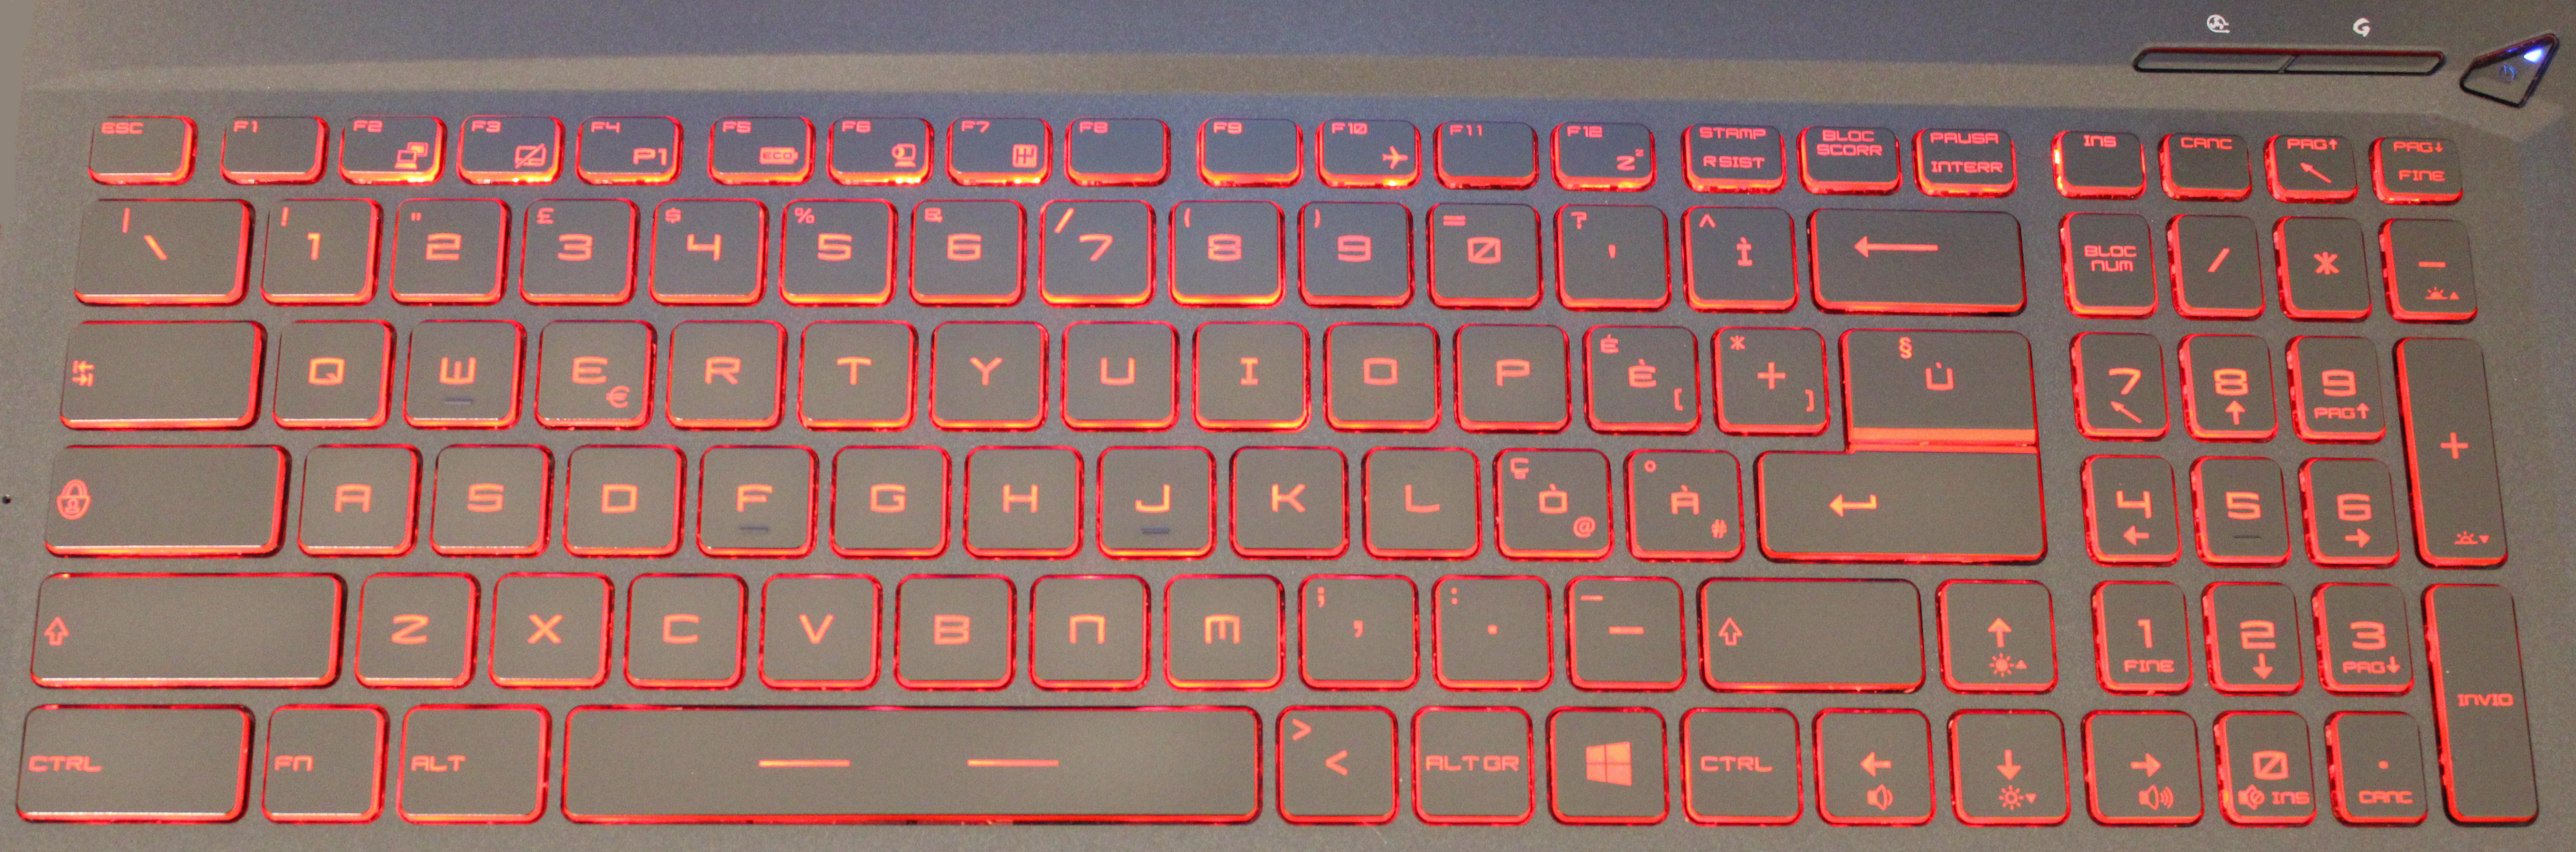
\includegraphics[width=.9\linewidth]{Images/KeyMapping/keyboard}
     \caption{\footnotesize{Layout of the keyboard of my MSI GL63 8RD laptop.}}\label{keymapping:keyboard}
\end{figure}

\begin{longtable}{cccc}
\hline
\textbf{key} & \textbf{real label} & \textbf{key-logger label} & \textbf{final label}\\
\hline
\begin{minipage}[c]{.3\textwidth}
\vspace{0.2cm}
\includegraphics[scale=0.1]{Images/KeyMapping/0}
\vspace{0.2cm}
\end{minipage} & & & 0 \\
\hline
\begin{minipage}[c]{.3\textwidth}
\vspace{0.2cm}
\includegraphics[scale=0.1]{Images/KeyMapping/0_INSERT}
\vspace{0.2cm}
\end{minipage} & & & 0\_INSERT\\
\hline
\begin{minipage}[c]{.3\textwidth}
\vspace{0.2cm}
\includegraphics[scale=0.1]{Images/KeyMapping/1}
\vspace{0.2cm}
\end{minipage} & & & 1\\
\hline
\begin{minipage}[c]{.3\textwidth}
\vspace{0.2cm}
\includegraphics[scale=0.1]{Images/KeyMapping/1_END}
\vspace{0.2cm}
\end{minipage} & & & 1\_END\\
\hline
\begin{minipage}[c]{.3\textwidth}
\vspace{0.2cm}
\includegraphics[scale=0.1]{Images/KeyMapping/2}
\vspace{0.2cm}
\end{minipage} & & & 2\\
\hline
\begin{minipage}[c]{.3\textwidth}
\vspace{0.2cm}
\includegraphics[scale=0.1]{Images/KeyMapping/2_DOWN}
\vspace{0.2cm}
\end{minipage} & & & 2\_DOWN\\
\hline
\begin{minipage}[c]{.3\textwidth}
\vspace{0.2cm}
\includegraphics[scale=0.1]{Images/KeyMapping/3}
\vspace{0.2cm}
\end{minipage} & & & 3\\
\hline
\begin{minipage}[c]{.3\textwidth}
\vspace{0.2cm}
\includegraphics[scale=0.1]{Images/KeyMapping/3_PAGE_DOWN}
\vspace{0.2cm}
\end{minipage} & & & 3\_PAGE\_DOWN\\
\hline
\begin{minipage}[c]{.3\textwidth}
\vspace{0.2cm}
\includegraphics[scale=0.1]{Images/KeyMapping/4}
\vspace{0.2cm}
\end{minipage} & & & 4\\
\hline
\begin{minipage}[c]{.3\textwidth}
\vspace{0.2cm}
\includegraphics[scale=0.1]{Images/KeyMapping/4_LEFT}
\vspace{0.2cm}
\end{minipage} & & & 4\_LEFT\\
\hline
\begin{minipage}[c]{.3\textwidth}
\vspace{0.2cm}
\includegraphics[scale=0.1]{Images/KeyMapping/5}
\vspace{0.2cm}
\end{minipage} & & & 5\\
\hline
\begin{minipage}[c]{.3\textwidth}
\vspace{0.2cm}
\includegraphics[scale=0.1]{Images/KeyMapping/5_NUM}
\vspace{0.2cm}
\end{minipage} & & & 5\_NUM\\
\hline
\begin{minipage}[c]{.3\textwidth}
\vspace{0.2cm}
\includegraphics[scale=0.1]{Images/KeyMapping/6}
\vspace{0.2cm}
\end{minipage} & & & 6\\
\hline
\begin{minipage}[c]{.3\textwidth}
\vspace{0.2cm}
\includegraphics[scale=0.1]{Images/KeyMapping/6_RIGHT}
\vspace{0.2cm}
\end{minipage} & & & 6\_RIGHT\\
\hline
\begin{minipage}[c]{.3\textwidth}
\vspace{0.2cm}
\includegraphics[scale=0.1]{Images/KeyMapping/7}
\vspace{0.2cm}
\end{minipage} & & & 7\\
\hline
\begin{minipage}[c]{.3\textwidth}
\vspace{0.2cm}
\includegraphics[scale=0.1]{Images/KeyMapping/7_HOME}
\vspace{0.2cm}
\end{minipage} & & & 7\_HOME\\
\hline
\begin{minipage}[c]{.3\textwidth}
\vspace{0.2cm}
\includegraphics[scale=0.1]{Images/KeyMapping/8}
\vspace{0.2cm}
\end{minipage} & & & 8\\
\hline
\begin{minipage}[c]{.3\textwidth}
\vspace{0.2cm}
\includegraphics[scale=0.1]{Images/KeyMapping/8_UP}
\vspace{0.2cm}
\end{minipage} & & & 8\_UP\\
\hline
\begin{minipage}[c]{.3\textwidth}
\vspace{0.2cm}
\includegraphics[scale=0.1]{Images/KeyMapping/9}
\vspace{0.2cm}
\end{minipage} & & & 9\\
\hline
\begin{minipage}[c]{.3\textwidth}
\vspace{0.2cm}
\includegraphics[scale=0.1]{Images/KeyMapping/9_PAGE_UP}
\vspace{0.2cm}
\end{minipage} & & & 9\_PAGE\_UP\\
\hline
\begin{minipage}[c]{.3\textwidth}
\vspace{0.2cm}
\includegraphics[scale=0.1]{Images/KeyMapping/a}
\vspace{0.2cm}
\end{minipage} & & & a\\
\hline
\begin{minipage}[c]{.3\textwidth}
\vspace{0.2cm}
\includegraphics[scale=0.1]{Images/KeyMapping/ALT}
\vspace{0.2cm}
\end{minipage} & & & ALT\\
\hline
\begin{minipage}[c]{.3\textwidth}
\vspace{0.2cm}
\includegraphics[scale=0.1]{Images/KeyMapping/ALT_GR}
\vspace{0.2cm}
\end{minipage} & & & ALT\_GR\\
\hline
\begin{minipage}[c]{.3\textwidth}
\vspace{0.2cm}
\includegraphics[scale=0.1]{Images/KeyMapping/APOSTROPHE}
\vspace{0.2cm}
\end{minipage} & & & APOSTROPHE\\
\hline
\begin{minipage}[c]{.3\textwidth}
\vspace{0.2cm}
\includegraphics[scale=0.1]{Images/KeyMapping/b}
\vspace{0.2cm}
\end{minipage} & & & b\\
\hline
\begin{minipage}[c]{.3\textwidth}
\vspace{0.2cm}
\includegraphics[scale=0.1]{Images/KeyMapping/BACKSLASH}
\vspace{0.2cm}
\end{minipage} & & & BACKSLASH\\
\hline
\begin{minipage}[c]{.3\textwidth}
\vspace{0.2cm}
\includegraphics[scale=0.1]{Images/KeyMapping/BACKSPACE}
\vspace{0.2cm}
\end{minipage} & & & BACKSPACE\\
\hline
\begin{minipage}[c]{.3\textwidth}
\vspace{0.2cm}
\includegraphics[scale=0.1]{Images/KeyMapping/c}
\vspace{0.2cm}
\end{minipage} & & & c\\
\hline
\begin{minipage}[c]{.3\textwidth}
\vspace{0.2cm}
\includegraphics[scale=0.1]{Images/KeyMapping/CAPS_LOCK}
\vspace{0.2cm}
\end{minipage} & & & CAPS\_LOCK\\
\hline
\begin{minipage}[c]{.3\textwidth}
\vspace{0.2cm}
\includegraphics[scale=0.1]{Images/KeyMapping/COMMA}
\vspace{0.2cm}
\end{minipage} & & & COMMA\\
\hline
\begin{minipage}[c]{.3\textwidth}
\vspace{0.2cm}
\includegraphics[scale=0.1]{Images/KeyMapping/CTRL}
\vspace{0.2cm}
\end{minipage} & & & CTRL\\
\hline
\begin{minipage}[c]{.3\textwidth}
\vspace{0.2cm}
\includegraphics[scale=0.1]{Images/KeyMapping/CTRL_R}
\vspace{0.2cm}
\end{minipage} & & & CTRL\_R\\
\hline
\begin{minipage}[c]{.3\textwidth}
\vspace{0.2cm}
\includegraphics[scale=0.1]{Images/KeyMapping/d}
\vspace{0.2cm}
\end{minipage} & & & d\\
\hline
\begin{minipage}[c]{.3\textwidth}
\vspace{0.2cm}
\includegraphics[scale=0.1]{Images/KeyMapping/DELETE}
\vspace{0.2cm}
\end{minipage} & & & DELETE\\
\hline
\begin{minipage}[c]{.3\textwidth}
\vspace{0.2cm}
\includegraphics[scale=0.1]{Images/KeyMapping/DOWN}
\vspace{0.2cm}
\end{minipage} & & & DOWN\\
\hline
\begin{minipage}[c]{.3\textwidth}
\vspace{0.2cm}
\includegraphics[scale=0.1]{Images/KeyMapping/e}
\vspace{0.2cm}
\end{minipage} & & & e\\
\hline
\begin{minipage}[c]{.3\textwidth}
\vspace{0.2cm}
\includegraphics[scale=0.1]{Images/KeyMapping/ENTER}
\vspace{0.2cm}
\end{minipage} & & & ENTER\\
\hline
\begin{minipage}[c]{.3\textwidth}
\vspace{0.2cm}
\includegraphics[scale=0.1]{Images/KeyMapping/ENTER_R}
\vspace{0.2cm}
\end{minipage} & & & ENTER\_R\\
\hline
\begin{minipage}[c]{.3\textwidth}
\vspace{0.2cm}
\includegraphics[scale=0.1]{Images/KeyMapping/ESC}
\vspace{0.2cm}
\end{minipage} & & & ESC\\
\hline
\begin{minipage}[c]{.3\textwidth}
\vspace{0.2cm}
\includegraphics[scale=0.1]{Images/KeyMapping/f}
\vspace{0.2cm}
\end{minipage} & & & f\\
\hline
\begin{minipage}[c]{.3\textwidth}
\vspace{0.2cm}
\includegraphics[scale=0.1]{Images/KeyMapping/F1}
\vspace{0.2cm}
\end{minipage} & & & F1\\
\hline
\begin{minipage}[c]{.3\textwidth}
\vspace{0.2cm}
\includegraphics[scale=0.1]{Images/KeyMapping/F10}
\vspace{0.2cm}
\end{minipage} & & & F10\\
\hline
\begin{minipage}[c]{.3\textwidth}
\vspace{0.2cm}
\includegraphics[scale=0.1]{Images/KeyMapping/F11}
\vspace{0.2cm}
\end{minipage} & & & F11\\
\hline
\begin{minipage}[c]{.3\textwidth}
\vspace{0.2cm}
\includegraphics[scale=0.1]{Images/KeyMapping/F12}
\vspace{0.2cm}
\end{minipage} & & & F12\\
\hline
\begin{minipage}[c]{.3\textwidth}
\vspace{0.2cm}
\includegraphics[scale=0.1]{Images/KeyMapping/F2}
\vspace{0.2cm}
\end{minipage} & & & F2\\
\hline
\begin{minipage}[c]{.3\textwidth}
\vspace{0.2cm}
\includegraphics[scale=0.1]{Images/KeyMapping/F3}
\vspace{0.2cm}
\end{minipage} & & & F3\\
\hline
\begin{minipage}[c]{.3\textwidth}
\vspace{0.2cm}
\includegraphics[scale=0.1]{Images/KeyMapping/F4}
\vspace{0.2cm}
\end{minipage} & & & F4\\
\hline
\begin{minipage}[c]{.3\textwidth}
\vspace{0.2cm}
\includegraphics[scale=0.1]{Images/KeyMapping/F5}
\vspace{0.2cm}
\end{minipage} & & & F5\\
\hline
\begin{minipage}[c]{.3\textwidth}
\vspace{0.2cm}
\includegraphics[scale=0.1]{Images/KeyMapping/F6}
\vspace{0.2cm}
\end{minipage} & & & F6\\
\hline
\begin{minipage}[c]{.3\textwidth}
\vspace{0.2cm}
\includegraphics[scale=0.1]{Images/KeyMapping/F7}
\vspace{0.2cm}
\end{minipage} & & & F7\\
\hline
\begin{minipage}[c]{.3\textwidth}
\vspace{0.2cm}
\includegraphics[scale=0.1]{Images/KeyMapping/F8}
\vspace{0.2cm}
\end{minipage} & & & F8\\
\hline
\begin{minipage}[c]{.3\textwidth}
\vspace{0.2cm}
\includegraphics[scale=0.1]{Images/KeyMapping/F9}
\vspace{0.2cm}
\end{minipage} & & & F9\\
\hline
\begin{minipage}[c]{.3\textwidth}
\vspace{0.2cm}
\includegraphics[scale=0.1]{Images/KeyMapping/FN}
\vspace{0.2cm}
\end{minipage} & & & FN\\
\hline
\begin{minipage}[c]{.3\textwidth}
\vspace{0.2cm}
\includegraphics[scale=0.1]{Images/KeyMapping/g}
\vspace{0.2cm}
\end{minipage} & & & g\\
\hline
\begin{minipage}[c]{.3\textwidth}
\vspace{0.2cm}
\includegraphics[scale=0.1]{Images/KeyMapping/h}
\vspace{0.2cm}
\end{minipage} & & & h\\
\hline
\begin{minipage}[c]{.3\textwidth}
\vspace{0.2cm}
\includegraphics[scale=0.1]{Images/KeyMapping/i}
\vspace{0.2cm}
\end{minipage} & & & i\\
\hline
\begin{minipage}[c]{.3\textwidth}
\vspace{0.2cm}
\includegraphics[scale=0.1]{Images/KeyMapping/INSERT}
\vspace{0.2cm}
\end{minipage} & & & INSERT\\
\hline
\begin{minipage}[c]{.3\textwidth}
\vspace{0.2cm}
\includegraphics[scale=0.1]{Images/KeyMapping/j}
\vspace{0.2cm}
\end{minipage} & & & j\\
\hline
\begin{minipage}[c]{.3\textwidth}
\vspace{0.2cm}
\includegraphics[scale=0.1]{Images/KeyMapping/k}
\vspace{0.2cm}
\end{minipage} & & & k\\
\hline
\begin{minipage}[c]{.3\textwidth}
\vspace{0.2cm}
\includegraphics[scale=0.1]{Images/KeyMapping/l}
\vspace{0.2cm}
\end{minipage} & & & l\\
\hline
\begin{minipage}[c]{.3\textwidth}
\vspace{0.2cm}
\includegraphics[scale=0.1]{Images/KeyMapping/LEFT}
\vspace{0.2cm}
\end{minipage} & & & LEFT\\
\hline
\begin{minipage}[c]{.3\textwidth}
\vspace{0.2cm}
\includegraphics[scale=0.1]{Images/KeyMapping/LOWER}
\vspace{0.2cm}
\end{minipage} & & & LOWER\\
\hline
\begin{minipage}[c]{.3\textwidth}
\vspace{0.2cm}
\includegraphics[scale=0.1]{Images/KeyMapping/m}
\vspace{0.2cm}
\end{minipage} & & & m\\
\hline
\begin{minipage}[c]{.3\textwidth}
\vspace{0.2cm}
\includegraphics[scale=0.1]{Images/KeyMapping/MINUS}
\vspace{0.2cm}
\end{minipage} & & & MINUS\\
\hline
\begin{minipage}[c]{.3\textwidth}
\vspace{0.2cm}
\includegraphics[scale=0.1]{Images/KeyMapping/MINUS_R}
\vspace{0.2cm}
\end{minipage} & & & MINUS\_R\\
\hline
\begin{minipage}[c]{.3\textwidth}
\vspace{0.2cm}
\includegraphics[scale=0.1]{Images/KeyMapping/n}
\vspace{0.2cm}
\end{minipage} & & & n\\
\hline
\begin{minipage}[c]{.3\textwidth}
\vspace{0.2cm}
\includegraphics[scale=0.1]{Images/KeyMapping/NUM_LOCK}
\vspace{0.2cm}
\end{minipage} & & & NUM\_LOCK\\
\hline
\begin{minipage}[c]{.3\textwidth}
\vspace{0.2cm}
\includegraphics[scale=0.1]{Images/KeyMapping/o}
\vspace{0.2cm}
\end{minipage} & & & o\\
\hline
\begin{minipage}[c]{.3\textwidth}
\vspace{0.2cm}
\includegraphics[scale=0.1]{Images/KeyMapping/p}
\vspace{0.2cm}
\end{minipage} & & & p\\
\hline
\begin{minipage}[c]{.3\textwidth}
\vspace{0.2cm}
\includegraphics[scale=0.1]{Images/KeyMapping/PAGE_DOWN}
\vspace{0.2cm}
\end{minipage} & & & PAGE\_DOWN\\
\hline
\begin{minipage}[c]{.3\textwidth}
\vspace{0.2cm}
\includegraphics[scale=0.1]{Images/KeyMapping/PAGE_UP}
\vspace{0.2cm}
\end{minipage} & & & PAGE\_UP\\
\hline
\begin{minipage}[c]{.3\textwidth}
\vspace{0.2cm}
\includegraphics[scale=0.1]{Images/KeyMapping/PAUSE}
\vspace{0.2cm}
\end{minipage} & & & PAUSE\\
\hline
\begin{minipage}[c]{.3\textwidth}
\vspace{0.2cm}
\includegraphics[scale=0.1]{Images/KeyMapping/PLUS}
\vspace{0.2cm}
\end{minipage} & & & PLUS\\
\hline
\begin{minipage}[c]{.3\textwidth}
\vspace{0.2cm}
\includegraphics[scale=0.1]{Images/KeyMapping/PLUS_R}
\vspace{0.2cm}
\end{minipage} & & & PLUS\_R\\
\hline
\begin{minipage}[c]{.3\textwidth}
\vspace{0.2cm}
\includegraphics[scale=0.1]{Images/KeyMapping/POINT}
\vspace{0.2cm}
\end{minipage} & & & POINT\\
\hline
\begin{minipage}[c]{.3\textwidth}
\vspace{0.2cm}
\includegraphics[scale=0.1]{Images/KeyMapping/POINT_DELETE}
\vspace{0.2cm}
\end{minipage} & & & POINT\_DELETE\\
\hline
\begin{minipage}[c]{.3\textwidth}
\vspace{0.2cm}
\includegraphics[scale=0.1]{Images/KeyMapping/PRINT_SCREEN}
\vspace{0.2cm}
\end{minipage} & & & PRINT\_SCREEN\\
\hline
\begin{minipage}[c]{.3\textwidth}
\vspace{0.2cm}
\includegraphics[scale=0.1]{Images/KeyMapping/q}
\vspace{0.2cm}
\end{minipage} & & & q\\
\hline
\begin{minipage}[c]{.3\textwidth}
\vspace{0.2cm}
\includegraphics[scale=0.1]{Images/KeyMapping/r}
\vspace{0.2cm}
\end{minipage} & & & r\\
\hline
\begin{minipage}[c]{.3\textwidth}
\vspace{0.2cm}
\includegraphics[scale=0.1]{Images/KeyMapping/RIGHT}
\vspace{0.2cm}
\end{minipage} & & & RIGHT\\
\hline
\begin{minipage}[c]{.3\textwidth}
\vspace{0.2cm}
\includegraphics[scale=0.1]{Images/KeyMapping/s}
\vspace{0.2cm}
\end{minipage} & & & s\\
\hline
\begin{minipage}[c]{.3\textwidth}
\vspace{0.2cm}
\includegraphics[scale=0.1]{Images/KeyMapping/SCROLL_LOCK}
\vspace{0.2cm}
\end{minipage} & & & SCROLL\_LOCK\\
\hline
\begin{minipage}[c]{.3\textwidth}
\vspace{0.2cm}
\includegraphics[scale=0.1]{Images/KeyMapping/SHIFT}
\vspace{0.2cm}
\end{minipage} & & & SHIFT\\
\hline
\begin{minipage}[c]{.3\textwidth}
\vspace{0.2cm}
\includegraphics[scale=0.1]{Images/KeyMapping/SHIFT_R}
\vspace{0.2cm}
\end{minipage} & & & SHIFT\_R\\
\hline
\begin{minipage}[c]{.3\textwidth}
\vspace{0.2cm}
\includegraphics[scale=0.1]{Images/KeyMapping/SLASH}
\vspace{0.2cm}
\end{minipage} & & & SLASH\\
\hline
\begin{minipage}[c]{.3\textwidth}
\vspace{0.2cm}
\includegraphics[scale=0.1]{Images/KeyMapping/SPACE}
\vspace{0.2cm}
\end{minipage} & & & SPACE\\
\hline
\begin{minipage}[c]{.3\textwidth}
\vspace{0.2cm}
\includegraphics[scale=0.1]{Images/KeyMapping/STAR}
\vspace{0.2cm}
\end{minipage} & & & STAR\\
\hline
\begin{minipage}[c]{.3\textwidth}
\vspace{0.2cm}
\includegraphics[scale=0.1]{Images/KeyMapping/t}
\vspace{0.2cm}
\end{minipage} & & & t\\
\hline
\begin{minipage}[c]{.3\textwidth}
\vspace{0.2cm}
\includegraphics[scale=0.1]{Images/KeyMapping/TAB}
\vspace{0.2cm}
\end{minipage} & & & TAB\\
\hline
\begin{minipage}[c]{.3\textwidth}
\vspace{0.2cm}
\includegraphics[scale=0.1]{Images/KeyMapping/u}
\vspace{0.2cm}
\end{minipage} & & & u\\
\hline
\begin{minipage}[c]{.3\textwidth}
\vspace{0.2cm}
\includegraphics[scale=0.1]{Images/KeyMapping/UP}
\vspace{0.2cm}
\end{minipage} & & & UP\\
\hline
\begin{minipage}[c]{.3\textwidth}
\vspace{0.2cm}
\includegraphics[scale=0.1]{Images/KeyMapping/v}
\vspace{0.2cm}
\end{minipage} & & & v\\
\hline
\begin{minipage}[c]{.3\textwidth}
\vspace{0.2cm}
\includegraphics[scale=0.1]{Images/KeyMapping/w}
\vspace{0.2cm}
\end{minipage} & & & w\\
\hline
\begin{minipage}[c]{.3\textwidth}
\vspace{0.2cm}
\includegraphics[scale=0.1]{Images/KeyMapping/WINDOWS}
\vspace{0.2cm}
\end{minipage} & & & WINDOWS\\
\hline
\begin{minipage}[c]{.3\textwidth}
\vspace{0.2cm}
\includegraphics[scale=0.1]{Images/KeyMapping/x}
\vspace{0.2cm}
\end{minipage} & & & x\\
\hline
\begin{minipage}[c]{.3\textwidth}
\vspace{0.2cm}
\includegraphics[scale=0.1]{Images/KeyMapping/y}
\vspace{0.2cm}
\end{minipage} & & & y\\
\hline
\begin{minipage}[c]{.3\textwidth}
\vspace{0.2cm}
\includegraphics[scale=0.1]{Images/KeyMapping/z}
\vspace{0.2cm}
\end{minipage} & & & z\\
\hline
\begin{minipage}[c]{.3\textwidth}
\vspace{0.2cm}
\includegraphics[scale=0.1]{Images/KeyMapping/à}
\vspace{0.2cm}
\end{minipage} & & & à\\
\hline
\begin{minipage}[c]{.3\textwidth}
\vspace{0.2cm}
\includegraphics[scale=0.1]{Images/KeyMapping/è}
\vspace{0.2cm}
\end{minipage} & & & è\\
\hline
\begin{minipage}[c]{.3\textwidth}
\vspace{0.2cm}
\includegraphics[scale=0.1]{Images/KeyMapping/ì}
\vspace{0.2cm}
\end{minipage} & & & ì\\
\hline
\begin{minipage}[c]{.3\textwidth}
\vspace{0.2cm}
\includegraphics[scale=0.1]{Images/KeyMapping/ò}
\vspace{0.2cm}
\end{minipage} & & & ò\\
\hline
\begin{minipage}[c]{.3\textwidth}
\vspace{0.2cm}
\includegraphics[scale=0.1]{Images/KeyMapping/ù}
\vspace{0.2cm}
\end{minipage} & & & ù\\
\hline
\end{longtable}

\addcontentsline{toc}{chapter}{\bibname}
\begin{thebibliography}{9}
%Introduction
\myBibItem{text_audio}{Sarika Choudhary, Ritika Saroha, Yatan Dahiya, and Sachin Choudhary}{Understanding CAPTCHA: Text and Audio Based Captcha with its Applications}{International Journal of Advanced Research in Computer Science and Software Engineering, vol. 3(6), pp. 106-115, 2013}

%State of the Art
\myBibItem{types_CAPTCHA}{Darko Brodi\'c, Alessia Amelio, Radmila Jankovi\'c}{Exploring the influence of CAPTCHA types to the users response time by statistical analysis}{Multimedia Tools and Applications, vol. 77, pp. 12293–12329, 2017}

\myBibItem{survey_advanced_CAPTCHA}{Walid Khalifa Abdullah Hasan}{A Survey of Current Research on Captcha}{International Journal of Computer Science Education in Schools (IJCSES), vol. 7, pp. 141–157, 2016}

\myBibItem{usability_CAPTCHA}{Ruti Gafni, Idan Nagar}{CAPTCHA – Security affecting user experience}{Issues in Informing Science and Information Technology, vol. 13, pp. 63-77, 2016}

\myBibItem{usability_audio}{G. Sauer, J. Holman, J. Lazar, H. Hochheiser, and J. Feng}{Accessible privacy and security: A universally usable human-interaction proof tool}{Univers. Access Inf. Soc., vol. 9, no. 3, p. 239–248, Aug. 2010}

\myBibItem{improving_audio}{Jennifer Tam, Jiri Simsa, David Huggins-Daines, Luis von Ahn, Manuel Blum}{Improving Audio CAPTCHAs}{Symposium On Usable Privacy and Security (SOUPS), 2008}

\myBibItem{DeepCRACk}{William Aiken, Hyoungshick Kim}{POSTER: DeepCRACk: Using Deep Learning to Automatically CRack Audio CAPTCHAs}{Proceedings of the 2018 on Asia Conference on Computer and Communications Security (ASIACCS), 2018}

\myBibItem{break_audio}{Jennifer Tam, Jiri Simsa, Sean Hyde, Luis von Ahn}{Breaking audio CAPTCHAs}{Advances in Neural Information Processing Systems, pp. 1625–1632, 2009}

\myBibItem{game_CAPTCHA}{Manar Mohamed, Song Gao, Nitesh Saxena, Chengcui Zhang}{Dynamic cognitive  game  captcha  usability  and  detection  of  streaming-based  farming}{The Workshop on Usable Security (USEC), co-located with NDSS, 2014}

\myBibItem{survey_CAPTCHA}{Ved Prakash Singh, Preet Pal}{Survey of Different Types of CAPTCHA}{International Journal of Computer Science and Information Technologies (IJCSIT), vol. 5(2), 2014}

\myBibItem{FaceDCAPTCHA}{Goswami G, Powell BM, Vatsa M, Singh R, Noore A}{FaceDCAPTCHA: face detection based color image CAPTCHA}{Future Generation Computer Systems, vol. 31(2), pp. 59–69, 2014}

\myBibItem{Viola_Jones}{Wen-yao Lu, Ming Yang}{Face Detection Based on Viola-Jones Algorithm Applying Composite Features}{International Conference on Robots \& Intelligent System (ICRIS), pp. 82-85, 2019}

\myBibItem{MB_CAPTCHA}{Brian M. Powell, Abhishek Kumar, Jatin Thapar, Gaurav Goswami, Mayank Vatsa, Richa Singh, Afzel Noore}{A multibiometrics-based CAPTCHA for improved online security}{IEEE 8th International Conference on Biometrics Theory, Applications and Systems, 2016}

\myBibItem{math_CAPTCHA}{Carlos Javier Hernandez-Castro, Arturo Ribagorda}{Pitfalls in CAPTCHA design and implementation: The Math CAPTCHA, a case study}{Computers \& Security, vol. 29(1), pp. 141-157, 2010}

\myBibRef{sliding_CAPTCHA}{Luke Wroblewski}{https://www.lukew.com/ff/entry.asp?1138}{A Sliding Alternative to CAPTCHA?}{2010}

\myBibItem{OCR}{Silky Azad, Kiran Jain,}{Captcha: Attacks and weaknesses against OCR technology}{Global Journal of Computer Science and Technology, 2013}

\myBibItem{DECAPTCHA}{E. Bursztein, M. Martin, J. Mitchell}{Text-based CAPTCHA strengths and weaknesses}{Proc. 18th ACM Conference on Computer and Communications Security (CCS), pp. 125–138, 2011}

\myBibItem{Motion_CAPTCHA}{M. Shirali-Shahreza and S. Shirali-Shahreza}{Motion CAPTCHA}{2008 Conference on Human System Interactions, Krakow, pp. 1042-1044, 2008}

\myBibItem{video_attack}{Kameswara Rao Kavya Sri, Gnana Sai}{A Novel Video CAPTCHA Technique to Prevent BOT Attacks}{International Conference on Computational Modeling and  Security (CMS 2016), Procedia Computer  Science, vol. 85, pp. 236–240, 2016}

\myBibItem{video_desc}{K. A. Kluever, R. Zanibbi}{Balancing usability and security in a video captcha}{Proceedings of the 5th Symposium on Usable Privacy and Security, 2009}

\myBibItem{voice_CAPTCHA}{Omar Ahmed Hedaia, Ahmed Shawish, Hana Houssein, Hala Zayed}{Bio-CAPTCHA Voice-Based Authentication Technique for Better Security and Usability in Cloud Computing}{International Journal of Service Science Management Engineering and Technology, vol. 11(2), pp. 59-79, 2020}

\myBibItem{rtCAPTCHA}{Erkam Uzun, Simon Chung}{rtCaptcha: A Real-Time Captcha Based Liveness Detection System}{The Network and Distributed System Security Symposium (NDSS), Georgia Institute of Technology, 2018}

\myBibRef{break_text}{Vinay Shet}{https://security.googleblog.com/2014/12/are-you-robot-introducing-no-captcha.html}{Are you a robot? Introducing "No CAPTCHA reCAPTCHA"}{2014}

\bibitem{google}TehnoBlog, \href{https://tehnoblog.org/google-no-captcha-invisible-recaptcha-first-experience-results-review/}{"Google no Captcha + INVISIBLE reCaptcha–First Experience Results Review"}, \emph{2019}.

\myBibItem{break_google}{Suphannee Sivakorn, Jason Polakis, Angelos D. Keromytis}{I'm not a human: Breaking the Google reCAPTCHA}{Black Hat, pp. 1–12, 2016}

\myBibItem{CAPPCHA}{Meriem Guerar, Alessio Merlo, Mauro Migliardi}{Completely automated public physical test to tell computers and humans apart: A usability study on mobile devices}{Future Generation Computer Systems, vol. 82, pp. 617–630, 2018}

\myBibItem{CAPTCHA_attack_process}{Narges Roshanbin, James Miller}{A survey and analysis of current CAPTCHA approaches}{Journal of Web Engineering, vol. 12, issue 1–2, pp. 1–40, 2013}

%Invisible CAPPCHA
\myBibItem{Invisible_CAPPCHA}{Meriem Guerar, Alessio Merlo, Mauro Migliardi, Francesco Palmieri}{Invisible CAPPCHA: A usable mechanism to distinguish between malware and humans on the mobile IoT}{Computers \& Security, vol. 78, pp. 255–266, 2018}

%Side-channel
\myBibItem{side_leaks}{Shuo Chen, Rui Wang, XiaoFeng Wang, Kehuan Zhang}{Side-Channel Leaks in Web Applications: A Reality Today, a Challenge Tomorrow}{2010 IEEE Symposium on Security and Privacy, pp. 191-20, 2010}

\myBibItem{side_authentication}{Kazuo Sakiyama, Takanori Machida, Arisa Matsubara, Yunfeng Kuai, Yu-ichi Hayashi, Takaaki Mizuki, Noriyuki Miura, Makoto Nagata}{Authentication Using Side-Channel Information.}{IACR Cryptol. ePrint Arch., 2015, 834}

\end{thebibliography}
\chapter*{Acknowledgements}
Professor Migliardi\\

I would like to express my very great appreciation to Dr Guerar\\

I would like to express my gratitude to University of Padova for the study path I performed. The uncertainty about the future and the idea of being far from needed cyber security skills have become a stimulus to improve myself. I learn a lot and I got hooked on the programming, starting from zero level of it, thanks to the professors' professionalism and knowledge. During the last five years, I've changed and now I spend programming all my free time. Thanks to University because professors follow my thirst of knowledge and I grew up, living alone and really becoming an adult.\\

Thanks to staff,

Thanks to other company,\\

Thanks to my family\\

Thanks to my grandmother\\

Thanks to Cristina,\\

Thanks to Francesca,

Thanks to Davide,\\

Thanks to Giuseppe, Aurora, Alessia and Sara,\\

Thanks to Elia,\\

Thanks to Lorenzo,\\

\end{document}